\documentclass[12pt,a4paper]{article}

% --- Encoding and math ---
\usepackage[utf8]{inputenc}
\usepackage[T1]{fontenc}
\usepackage{amsmath,amssymb,amsthm}

% --- Graphics and layout ---
\usepackage{graphicx}
\usepackage{geometry}
\geometry{margin=1in}
\usepackage[expansion=false]{microtype}

% --- TikZ for figures ---
\usepackage{tikz}
\usetikzlibrary{arrows.meta, positioning, shapes, shadows, decorations.pathmorphing}
\def\wave{decorate, decoration={coil, aspect=0}}

% --- Tables ---
\usepackage{booktabs}

% --- Section formatting ---
\usepackage{titlesec}

% --- Floats, spacing, paragraph style ---
\usepackage{float}
\usepackage{setspace}
\usepackage{parskip}

% --- Verbatim with wrapping ---
\usepackage{fancyvrb}
\usepackage{fvextra}

% --- Numeric tables ---
\usepackage{siunitx}
\sisetup{
    table-number-alignment = center,
    table-text-alignment   = center
}

% --- Input path flexibility ---
\makeatletter
\def\input@path{{./}{./tables/}}
\makeatother

% --- Line spacing ---
\onehalfspacing

% --- Citations and links ---
\usepackage[authoryear]{natbib}
\usepackage{hyperref}
\hypersetup{
  colorlinks=true,
  linkcolor=black,
  citecolor=black,
  urlcolor=black
}

\title{Synthetic-Emotional Calibration (SEC):\\
\Large A Governed Control Interface for Stability and Viability \\
\large in Instrumented Cognitive Systems}

\author{John H. Cragin\\
Independent Researcher\\
john.cragin@outlook.com}

\date{\today{}}

\begin{document}

\maketitle

\begin{abstract}
Synthetic-Emotional Calibration (SEC) is introduced as a governed control interface that enables precise, inspectable modulation of regulatory behavior in cognitive systems prioritizing stability and viability. Unlike affective computing or reward-based approaches, SEC operates as a constraint mechanism, mapping discrete regulatory modes to calibrated parameter vectors that govern internal dynamics without persistent learning or external optimization. This paper formally defines the SEC formalism, including its vector representation, emoji-indexed calibration table, and control semantics, demonstrating how it functions as an externalized governance surface for safety-critical AI. By externalizing calibration parameters in a human-legible, auditable format, SEC supports reproducibility and architectural decoupling while explicitly limiting system behavior to ensure viability under uncertainty. The design is specific to instrumented cognitive architectures and should not be interpreted as a universal control mechanism or model of human emotion. This work provides the mechanistic foundation for SEC's role in regulatory intelligence, complementing system-level validations presented elsewhere.
\end{abstract}

\section{Introduction}

The problem: symbolic and hybrid systems lack a stable, inspectable internal regulation layer. Raw optimization signals (loss, reward, accuracy) are insufficient for viability, as they do not provide bounded, interpretable modulation of internal dynamics. This paper introduces Synthetic-Emotional Calibration (SEC) as a governed control interface for stability and viability in instrumented cognitive systems.

SEC defines a formal mapping between discrete regulatory modes and calibrated parameter vectors, enabling precise governance of system behavior without exposing implementation internals. This work specifies the SEC formalism, explains its representation and calibration mechanisms, and demonstrates how it serves as an inspectable control surface for viability-first AI.

The remainder of this paper defines SEC mechanistically, positions it within the regulatory intelligence paradigm, and outlines its governance properties.

\section{Background and Motivation}

From affective labels to regulatory signals. Affective computing approaches simulate human emotions for user interaction \cite{Picard2000}, but fail to provide governed internal regulation for cognitive stability. Reward shaping in reinforcement learning optimizes external objectives \cite{Sutton2018}, yet lacks the bounded modulation needed for viability under uncertainty. Prompt steering in large language models adjusts outputs through natural language, but does not constrain internal regulatory dynamics.

SEC's design goal is bounded, interpretable modulation of cognition, not expressive freedom. It addresses the need for a control interface that calibrates regulatory behavior without compromising non-learning constraints or architectural inspectability.

\section{Definition of Synthetic-Emotional Calibration}

What "calibration" means. SEC is a vector-valued function that maps discrete regulatory mode identifiers to calibrated parameter vectors, governing internal system modulation. It distinguishes between emotional representation (modeling affective states) and emotional calibration (adjusting regulatory controls).

SEC should not be interpreted as biological emotion, phenomenology, or sentiment analysis. It operates as a control formalism, not an affective model, explicitly constraining system behavior to ensure stability and viability \cite{Ashby1956,Aubin2009}.

\section{SEC Representation}

Vectors, anchors, and identifiers.

The SEC vector operates in a continuous affective space of calibrated parameters, with dimensions governing regulatory controls such as thresholds, gains, and sensitivities.

Discrete regulatory mode anchors provide stable reference points for transitions, each representing a coherent regulatory posture.

Symbolic identifiers, implemented as emoji tokens, offer semantic stability, human legibility, and machine invariance. Emojis serve as compact identifiers for modes, not emotional labels or communicative outputs, ensuring consistent mode recognition across contexts. In execution, SEC modes are resolved via Unicode code points rather than rendered glyphs, ensuring unambiguous, font-independent identification. The use of $\text{U+}XXXX$ identifiers ensures that the governance layer is invariant to front-end rendering, preventing semantic drift in head-less deployments.

\begin{figure}[H]
\centering
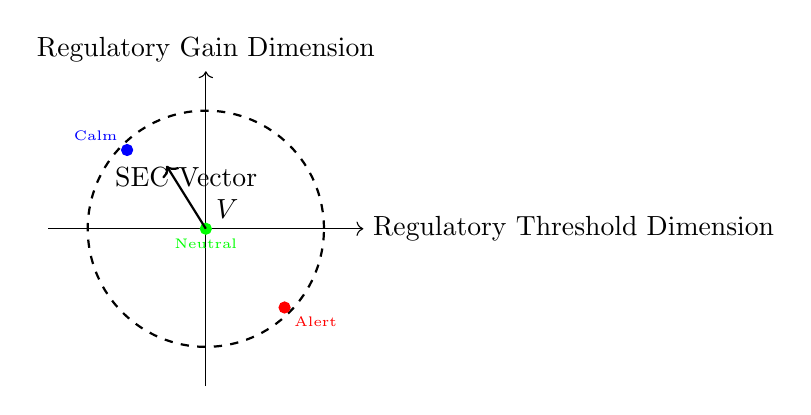
\begin{tikzpicture}
    % Draw a 2D plane for simplicity
    \draw[->] (-2,0) -- (2,0) node[right] {Regulatory Threshold Dimension};
    \draw[->] (0,-2) -- (0,2) node[above] {Regulatory Gain Dimension};
    
    % Viability Boundary
    \draw[dashed, thick] (0,0) ellipse (1.5 and 1.5) node[above right] {$V$};
    
    % Anchors
    \filldraw[blue] (-1,1) circle (2pt) node[above left] {\tiny Calm};
    \filldraw[red] (1,-1) circle (2pt) node[below right] {\tiny Alert};
    \filldraw[green] (0,0) circle (2pt) node[below] {\tiny Neutral};
    
    % Vector example
    \draw[thick,->] (0,0) -- (-0.5,0.8) node[midway,above] {SEC Vector};
\end{tikzpicture}
\caption{SEC Vector Space: Anchored regulatory modes in a continuous parameter space, bounded by the Viability Boundary ($V$) to ensure stability and viability. Axes and coordinates are schematic and illustrative, not exhaustive or implementation-specific.}
\label{fig:sec_vector}
\end{figure}

\begin{figure}[H]
\centering
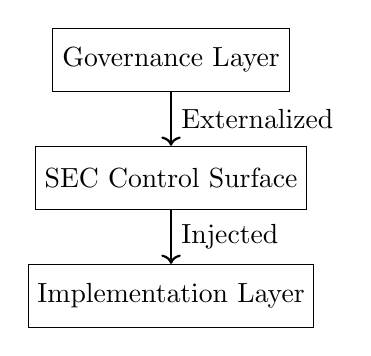
\begin{tikzpicture}
    % Governance Hierarchy
    \node[draw, rectangle, minimum width=3cm, minimum height=0.8cm] (gov) at (0,3) {Governance Layer};
    \node[draw, rectangle, minimum width=3cm, minimum height=0.8cm] (sec) at (0,1.5) {SEC Control Surface};
    \node[draw, rectangle, minimum width=3cm, minimum height=0.8cm] (impl) at (0,0) {Implementation Layer};
    
    % Arrows
    \draw[->, thick] (gov) -- (sec) node[midway, right] {Externalized};
    \draw[->, thick] (sec) -- (impl) node[midway, right] {Injected};
\end{tikzpicture}
\caption{Governance Surface Hierarchy: SEC functions as an externalized control interface, decoupling governance specifications from implementation details while enabling bounded modulation of internal dynamics.}
\label{fig:governance_hierarchy}
\end{figure}

\section{The Calibration Table (CSV) as a Control Artifact}

Why it is external, static, and inspectable.

The calibration table encodes mode identifiers, control parameter bounds, and allowed regulatory transitions in a static CSV format. It is not learned at runtime, not hard-coded logic, and not a natural language prompt.

This externalization enables reproducibility through version control, audit through human inspection, and safety by requiring explicit modifications for behavioral changes. The CSV serves as a governance surface, decoupling control specifications from implementation details.

Table~\ref{tab:sec_example} provides a schematic excerpt of the SEC calibration format for illustrative purposes only. Values are representative and intentionally incomplete; the full calibration table, transition constraints, and enforcement logic are not publicly released.

\begin{table}[H]
\centering
\footnotesize
\resizebox{\textwidth}{!}{%
\begin{tabular}{@{}lccccccccccccc@{}}
\toprule
codepoint & sec\_valence & sec\_arousal & sec\_intensity & alpha\_tgt & beta\_tgt & gamma\_tgt & delta\_tgt & H\_target & g\_pause & g\_reflect & g\_converge & tempo\_bucket & anchor \\
\midrule
U+1F6D1 & 0.50 & 0.35 & 0.40 & 0.18 & 0.18 & 0.23 & 0.32 & 2 & 1 & 0 & 0 & slow    & closure \\
U+1F504 & 0.50 & 0.50 & 0.50 & 0.24 & 0.23 & 0.29 & 0.26 & 4 & 0 & 0 & 1 & neutral & reflection \\
U+1F300 & 0.55 & 0.05 & 0.25 & 0.22 & 0.22 & 0.24 & 0.29 & 3 & 0 & 1 & 0 & slow    & analysis \\
U+1FAB6 & 0.50 & 0.35 & 0.40 & 0.22 & 0.22 & 0.24 & 0.29 & 3 & 0 & 1 & 0 & slow    & closure \\
U+26A1  & 0.30 & 1.00 & 0.90 & 0.27 & 0.27 & 0.24 & 0.24 & 4 & 0 & 0 & 0 & fast    & renewal \\
\bottomrule
\end{tabular}
} % end resizebox
\caption{Schematic excerpt of the SEC calibration table format. Each row specifies a calibrated 
regulatory posture rather than an emotional state. Emoji tokens are referenced by their Unicode 
code points (e.g., U+1F6D1), providing compact, human-legible identifiers for these postures, 
while numeric fields define bounded control targets and gating flags. The table is static and 
externally versioned; it does not encode learning, optimization, or transition logic. Multiple 
emoji tokens may map to similar regulatory anchors, enabling semantic redundancy without 
expanding the control space.}
\label{tab:sec_example}
\end{table}



\section{Control Semantics}

SEC modulates system behavior through parameter injection at regulatory decision points. The resolution process is schematized as follows:

\begin{verbatim}
Input: mode_identifier (Unicode code point)
Lookup: SEC[mode_identifier] → parameter_vector
Apply: parameter_vector → regulatory control points
Scope: single execution cycle (no persistence)
\end{verbatim}

\begin{itemize}
    \item \textbf{Threshold Modulation}: Risk tolerance boundaries are adjusted based on SEC vector components
    \item \textbf{Gain Control}: Regulatory feedback strengths are scaled by affective parameters
    \item \textbf{Pathway Coupling}: Inter-pathway interactions are weighted according to calibration values
    \item \textbf{Hazard Filtering}: Detection sensitivities are tuned to match regulatory posture
\end{itemize}

These modulations occur within a single execution cycle, with no persistent state changes across runs.

\section{Governance and Safety Properties}

Why this layer exists at all.

SEC provides inspectability through externalized parameters, version control for calibration tables, and a bounded action space that constrains regulatory dynamics \cite{Conant1970}. It exhibits fail-loud behavior by requiring explicit mode specifications and supports external validation.

Rather than amplifying emergent behavior, SEC limits system dynamics to ensure stability, functioning as a safety boundary for viability-first architectures.

\section{Relation to the Regulatory Intelligence Paradigm}

Where SEC sits in the larger system.

SEC serves as the physiological interface of the Regulatory Intelligence (RI) paradigm \cite{Cragin2025Monograph}, enabling calibrated modulation within geometric homeostasis and viability sets. It relates to intervention intelligence by providing the control surface for regulatory responses.

SEC does not define intelligence; it enables regulated intelligence by governing internal dynamics without persistent adaptation.

\section{Limitations and Non-Claims}

Explicitly tightening scope.

The SEC formalism is specific to SpiralBrain-class architectures and makes no universality claims. It does not claim optimality, psychological realism, or replacement for learned adaptation. This paper does not cover implementation details, empirical validations, or extensions beyond regulatory intelligence.

\section{Relation to Companion Works in the Regulatory Intelligence Corpus}

This paper specifies the formal structure and governance semantics of Synthetic-Emotional Calibration (SEC). Empirical evaluations, geometric analyses, and domain-specific applications are intentionally presented in separate companion works within the broader Regulatory Intelligence research corpus. Relevant extensions include:

\textbf{Phase Lock Optimization in Regulatory Cognitive Architectures} \\
Formal analysis of phase-lock dynamics and stability bounds within viability-first systems. \\
(See: \url{https://github.com/jhcragin/SpiralBrain-v3.0-public/tree/main/Phase Lock Optimization in Regulatory Cognitive Architectures}; Zenodo link forthcoming.)

\textbf{Bifurcation Points and Integrity Collapse in an Instrumented Cognitive System} \\
Empirical study of attractor collapse and recovery under regulatory stress. \\
(See: \url{https://github.com/jhcragin/SpiralBrain-v3.0-public/tree/main/bifurcation_integrity_collapse}; Zenodo link forthcoming.)

\textbf{Emotion as a Control Signal for Symbolic Stability} \\
Experimental validation of SEC-conditioned posture separation under identical inputs. \\
(See: \url{https://github.com/jhcragin/SpiralBrain-v3.0-public/tree/main/Emotion as a Control Signal for Symbolic Stability}; Zenodo link forthcoming.)

\textbf{Regulatory Asymmetries Under Scarcity} \\
Analysis of adaptive versus coercive regulation under matched scarcity regimes. \\
(See: \url{https://github.com/jhcragin/SpiralBrain-v3.0-public/tree/main/Regulatory Asymmetries Under Scarcity}; Zenodo link forthcoming.)

\textbf{The Regulatory Intelligence Paradigm: Geometric Homeostasis and Elastic Cognition} \\
Monograph defining the full theoretical framework in which SEC operates as a physiological control interface. \\
(See: \url{https://github.com/jhcragin/SpiralBrain-v3.0-public/tree/main/regulatory_intelligence_program}; Zenodo link forthcoming.)

These works expand upon SEC's role in stability, scarcity response, geometric homeostasis, and intervention intelligence, while the present paper remains focused on formal definition and governance semantics.

\section{Conclusion}

What this paper contributes.

This paper establishes SEC as a reusable control formalism for governed cognitive systems, specifying its representation, calibration, and governance properties. Explicit calibration surfaces like SEC are essential for inspectable, stable AI that prioritizes viability over optimization. Empirical validations of SEC's role in stability, scarcity response, and regulatory control are reported in companion works within the Regulatory Intelligence program. Companion validations demonstrate that SEC-conditioned regulation yields consistent posture separation under identical inputs and bounded drift under scarcity stress.

\section{Code Availability}

The experiments reported in this paper were conducted using the canonical SpiralBrain v3.0 configuration.
A public repository providing architectural documentation, configuration summaries, and reproducibility materials for this canonical configuration is available at: \\
\url{https://github.com/jhcragin/SpiralBrain-v3.0-public}. \\

The complete SpiralBrain codebase is not publicly available. Components beyond the public canonical configuration include research, experimental, and exploratory modules that were not exercised in the reported experiments and are maintained under a restricted research license.

A public repository accompanying this paper provides illustrative calibration excerpts and interface stubs demonstrating the SEC format and symbolic handling. These artifacts are schematic and non-executable, and do not include the full SpiralBrain implementation.

\bibliographystyle{plainnat}
\bibliography{references}

\end{document}